\setlength{\footskip}{8mm}

\chapter{Literature Review} 
\label{ch:literature-review}

This thesis chapter introduces concepts, technologies, techniques, consulted papers and articles pertaining to the core concepts of Customer Churn \& Retention, OLAP \& Datawarehouse, Data mining, Model evaluation metrics, Review of of selected papers and Summary of selected papers.

\section{Customer Churn \& Retention}
Customers are the most volatile asset of a services based company. Many frequently churn in search of better services. Customers are frivolous and those with prepaid or prepay plans are most unfaithful. Companies are generally in profit if they are able to retain customers and it pays off to almost six times \shortcite{bhatt1998custret}. Customers spending longer durations with a company are not easily churned and would not be affected by marketing strategies of rival companies. These customers are valuable to the company and generate profit in revenue. Research studies  have shown that long standing customers would be engaged in influencing newer customers to buy into a contract with their service provider \shortcite{mizerski1982}.\\
The ARPU of a stable customer is high compared to that of a churning customer. Thus marketing managers are focusing on advertising competitive products to retain customers from churning. The loss of capital due to a defecting customer is higher than the cost of retention. As per Forbes, Nov 11, 2013, earnings can swing positively by about 10 \% if customers are successfully retained.

\section{OLAP \& Datawarehouse }
Systems and companies are ever expanding. They are collecting data at unprecedented rates. Managing data becomes easier with the implementation of Data-warehouse. In many a cases the database of a company is segregated into different schema's. Segregation of schema's helps to avoid necessary access privileges and grants confusion. It also helps to maintain the organizational level of segregation in the database, ie., the HR department tables will be unaccessible to an accounts official and vice versa. But company leaders and decision makers should be accessing specific key counts and aggregations from all of their departments. A collection of tables sourcing data from their individual units.\\

OLAP - Online Analytical Processing is an extension of Data-warehouse technology \shortcite{han1997olap}. Olap consists of four main processes viz., Drill-down, Roll-up, slice and dice. Multi-demensional data can be fetched by OLAP from the Datawarehouse, and the unit of this is called the OLAP cube.There are two types of OLAP - MOLAP \& ROLAP. MOLAP Multidimensional OLAP is a solution used widely. 

One very famous open-source  OLAP solution is the Kylin\textsuperscript{TM} \shortcite{ApacheKylin}. Shown in Figure~\ref{fig:Kyline} is the architecture of the product.


\begin{figure}[h]
	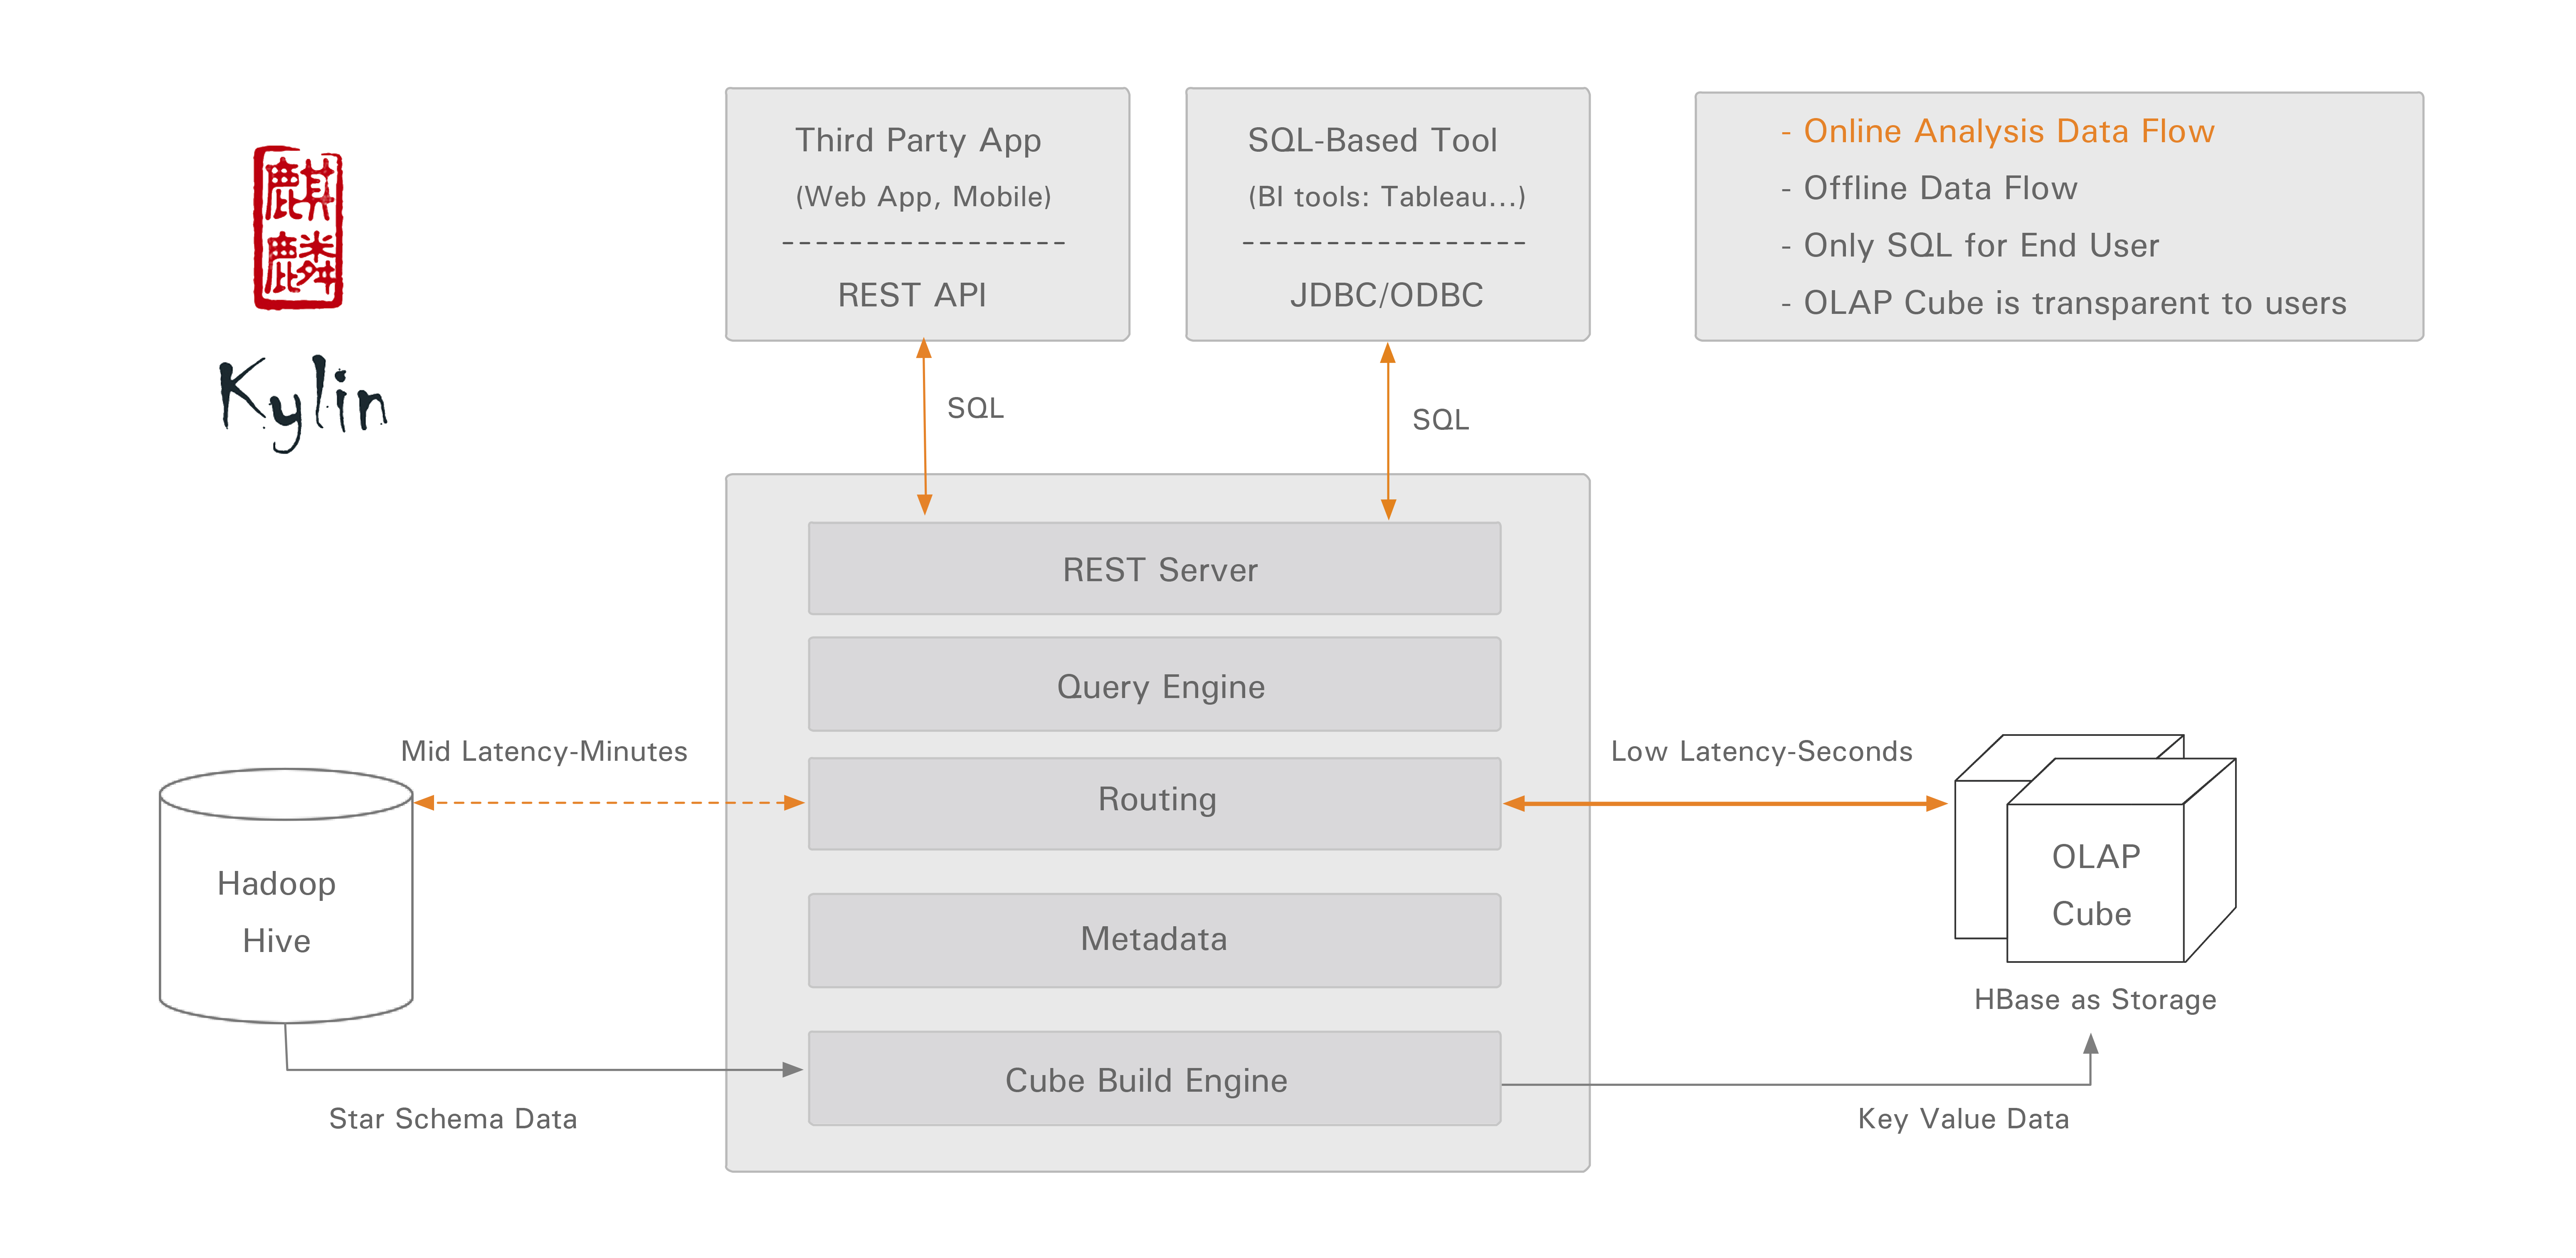
\includegraphics[width=\columnwidth,height=9cm]{figures/kylin_diagram.png}
	\centering
	\caption{OLAP Solution - Apache Kylin}
	\label{fig:Kyline}
\end{figure}


\section{Data Mining}
\label{data-mining}
Data mining is the process of extracting useful trend and patterns from structured and unstructured sources of data. Sometimes many academicians refer to it as KDD (Knowledge Discovery in Databases). John Naisbett (author of famous 'Megatrends') said \say{We are drowning in information but starved for knowledge.}
There are various techniques to perform data mining and these can be broadly classified into two categories Supervised Learning, Un-Supervised Learning.	
A very common terminology used in the data science field is of machine learning and it also used instead of data mining. 

\subsection{Supervised Learning}
This part of the data mining consists of classification and regression algorithms. Control and dependent variables of the given data are known entities. The use of these algorithms is to predict the outcome given past data. These algorithms have to be trained with a set of data and then they have to be tested. After reaching certain acceptable level of accuracy, these algorithms are used for prediction. 
\\
\\
Below are some of the Supervised learning techniques :
\begin{itemize}
	\item Linear regression : The prediction of dependent variable is done given the value of known variable. There is only 1 dependent variable. For example, \(y=\beta0 + \beta1x + \varepsilon\) \\
	y = dependent variable, 
	x = independent variable
	\item Multiple regression : is an extension of the linear regression but has more number of independent variables.
	\item Nonlinear regression : there are two variables but they are related in a curvilinear fashion i.e., not governed by the straight line equations.
	\item Logistic regression : A regression based modeling technique, which is better than linear regression when more variables are considered. Output variable is categorical in nature. 
	\item Decision tree : This is a classification algorithm which when plotted resembles an upside down tree structure. Given that a set of data has many attributes and there is a need to classify them, a decision tree is very suitable method to do so. There are many types of decision trees like the ID3, CART, C4.5 and C5.0. In Figure~\ref{fig:decisiontree} a simple DT for mammal classification model is shown. A decision tree can be designed using \textbf{Hunt's Algorithm}.
	\begin{figure}[H]
		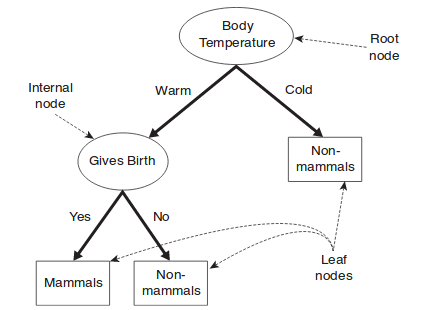
\includegraphics[scale=0.65]{figures/example_decisiontree.png}
		\centering
		\caption{Mammal classification problem}
		\label{fig:decisiontree}
	\end{figure}
	\item Random Forest : This technique can be used for both classification or regression type problems. A random forest is combination of many decision trees. In some cases random forest is sometimes very accurate.
	\item Support Vector Machine : This is a classifier technique where the data is segregated by generating hyperplanes. If there are n-features in the data then there have to be n-hyperplanes. The best classification is the hyperplane which clearly separates the data points.
	\item k-Nearest Neighbors : A learning algorithm that classifies the data into clusters nearest to them. The euclidean distance or manhattan distance could be some of the methods to find the nearest cluster. It is sometimes considered a lazy learning algorithm.
	\item Naive Bayes : This is an classification rule working on the probabilistic Bayes theorem.\newline
	 \(P(H|X) = P(X|H) P(H)/P(X)\).\newline
	\item Artificial neural networks : Neural networks are classification methods modeled after neurons \shortcite{neuralnetwork}. There are many layers with nodes Figure~\ref{fig:neuralnet}. There are many types of neural networks viz., Feed Forward NN, Radial Bias function, Recurrent NN, Backpropagation NN, Perceptron etc. Neural networks are very fast learners.
	\begin{figure}[H]
		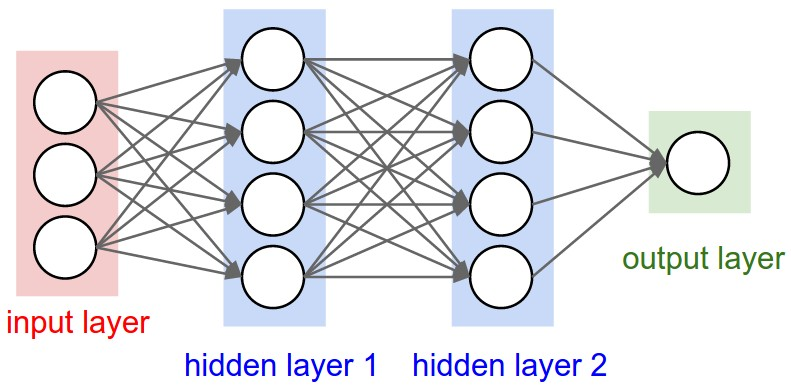
\includegraphics[scale = 0.5]{figures/neural_net2.jpeg}
		\centering
		\caption{A sample neural network}
		\label{fig:neuralnet}
	\end{figure}
\end{itemize}

\subsection{Un-Supervised Learning}
The clustering and association techniques in data mining are grouped into Un-Supervised learning. The output variables are not known.
Below are some Unsupervised class of algorithms :
\begin{itemize}
	\item K-means clustering : it is a means of clustering a set of data points with some k centroids. For each data point the distance is calculated and the nearest centroid is chosen and data point is associated with that cluster. After every iteration of cluster formation a new centroid is calculated and the distance of the data points are taken. The clusters are reformed and the iteration is performed till no data point movement happens.
	\item Apriori clustering : Here in the A priori algorithm is used to create the clusters. A priori is used for frequent item set mining states that sets of items are frequent if the items themselves are frequent. 
	\item Hierarchical clustering : This is a clustering method in which large clusters are further segregated into smaller clusters. This is the Divisive type of HC. In the Agglomerative type of HC, the nearby clusters are joined to form larger clusters. A Dendogram is used to graphically represent the clusters.	
	\item Hidden Markov models : These are used to analyze or predict time series problems in fields of speech, language, medicine, and robotics. Core of the technique is formed on the foundations of Bayes Network. In a markov chain a future state depends only on the current state. It is called Hidden because only certain measurements can be see of the states, not the states itself. Particle filter and Kalman filter are HMM's.
	\item Self organizing maps (SOM) : This is a type of neural network. Types are of Vector Quantizer or Kohonen SOM. In Figure~\ref{fig:kohonen} is an illustration of an Kohonen SOM.
		\begin{figure}[H]
			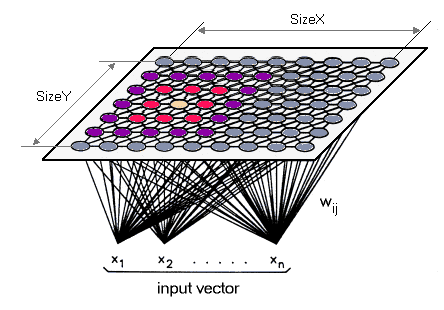
\includegraphics[scale = 1]{figures/Kohonen.png}
			\centering
			\caption{Kohonen SOM}
			\label{fig:kohonen}
		\end{figure}
\end{itemize}

\newpage
\subsection{Selecting the Right technique}
It is of utmost importance that a data scientist select the important mining  technique. Of all the process involved in the knowledge discovery process, selection of algorithm is quite difficult. Figure \ref{fig:selectdatamining},  from ``Choosing the Right Data Mining Technique: Classification of Methods and Intelligent Recommendation''  \shortcite{gibert2010choosing} shows the approach which could be taken to select between the various models available for data mining.

\begin{figure}[H]
	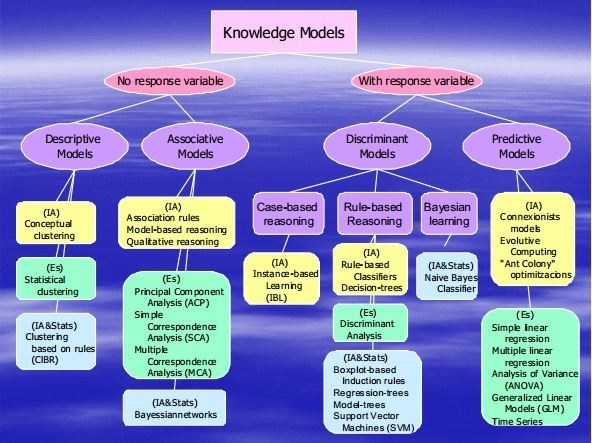
\includegraphics[width=\columnwidth,height=10cm]{figures/selectionofdatamining.jpeg}
	\centering
	\caption{Select the Right Mining Technique }
	\label{fig:selectdatamining}
\end{figure}

In addition to the above there is another approach, shown in Figure \ref{fig:scikit} suggested by the very popular scikit (machine learning library) of python for data mining \shortcite{scikitpython}.

\begin{figure}[H]
	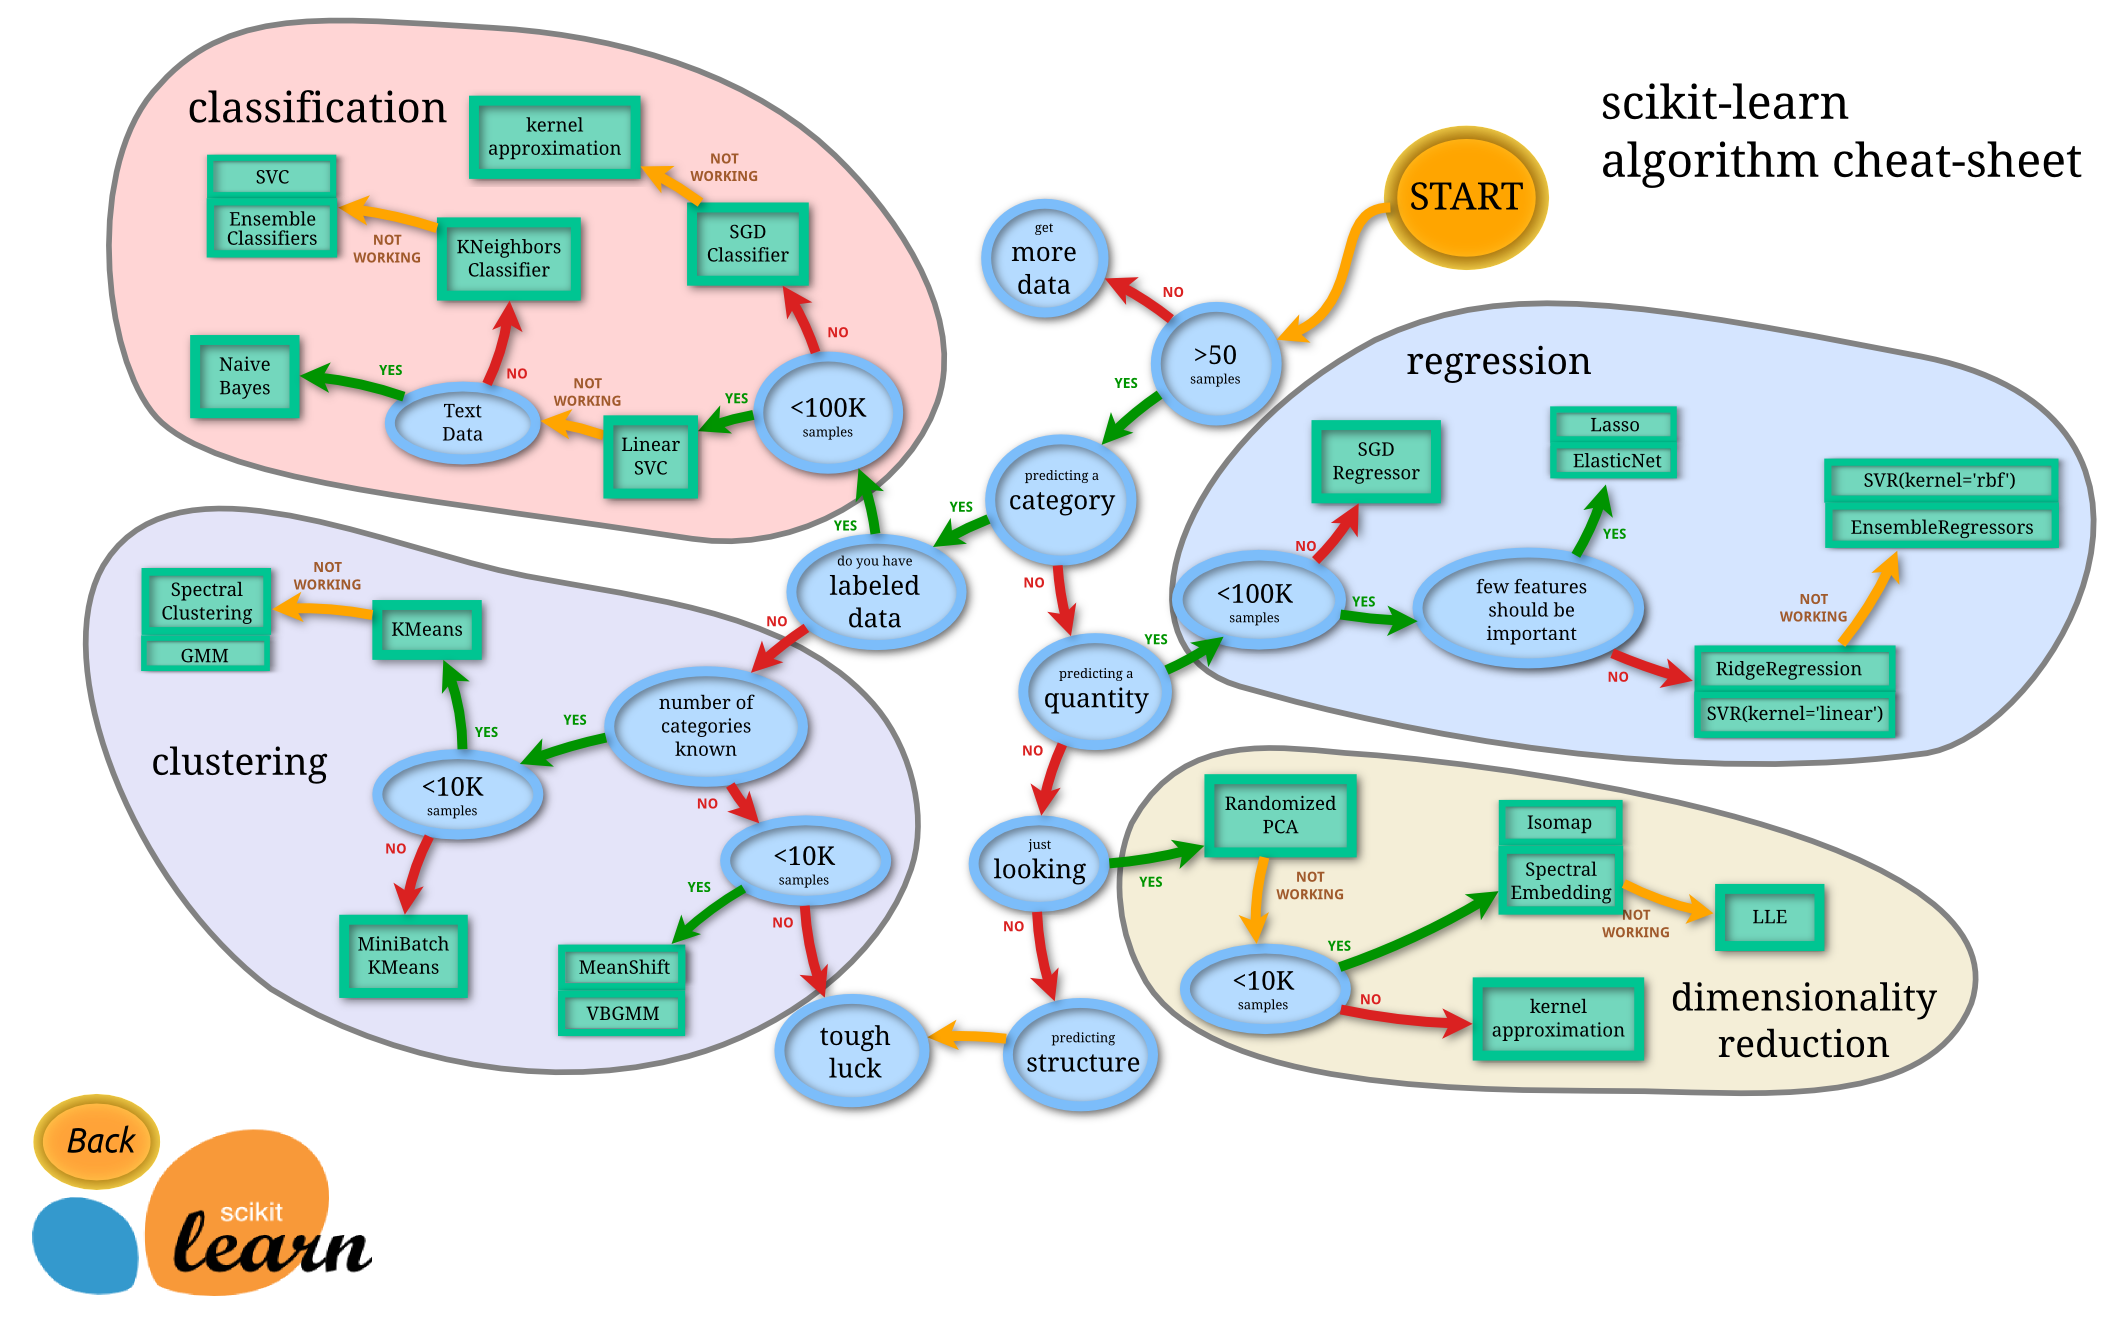
\includegraphics[width=\columnwidth,height=12cm]{figures/scikitlearn.png}
	\centering
	\caption{Another approach to select the Data Mining. Reprinted from Scikit}
	\label{fig:scikit}
\end{figure}


\subsection{Softwares, Libraries and Servers} 
Data mining techniques have been implemented into modules by a number of generous  contributers. There are some very famous solutions that an academician can utilize for implementing predictive analytics. The algorithms and techniques of neural networks, clustering, classification ans associations are available as solutions and API's. Following is a list in no particular order:
\begin{itemize}
	\item Softwares : The following softwares are open source and available for data analytics by downloading to the desktop.
	\begin{itemize}
		\item Weka : This is a open source software containing data mining algorithms. This can be used as a software or called by users own Java code.
		\item Knime : An open source tool for data mining, comprises of many functions from data cleaning to pattern analysis.
		\item Rapidminer : Also another popular tool for machine learning with plenty of algorithms for analysis.
	\end{itemize}
	\item Libraries : These are available for use as toolbox and academic can program own solution.
	\begin{itemize}
		\item Tensorflow
		\item mlpack
		\item H2O
		\item Mlib
		\item Scikit
	\end{itemize}
	\item Servers : The following servers have built in modules that can be accessed via web applications and can be modeled to process real time analytics instead of one of processing as with above solutions
	\begin{itemize}
		\item \textbf{DeepDetect} : is an open source deep learning server implemented in C++. It can be supported with back end machine learning applications with TensorFlow XGBoost and Caffe. Model assessment is built in the framework.
		\item \textbf{Apache Prediction IO} : This a open source stack for academicians to deploy machine learning. The stack has an Event Server that can be used to query from a web application and respond in real time. The Event server co-ordinates with the Engine to respond to API inputs and respond with predicted outcomes Figure \ref{fig:predictionio} \shortcite{PredictionIO}. PredictionIO provides various templates for varied mining algorithms. Classification templates like Decision trees, Logistic Reressiong, NLP are available for use.
		\begin{figure}[H]
			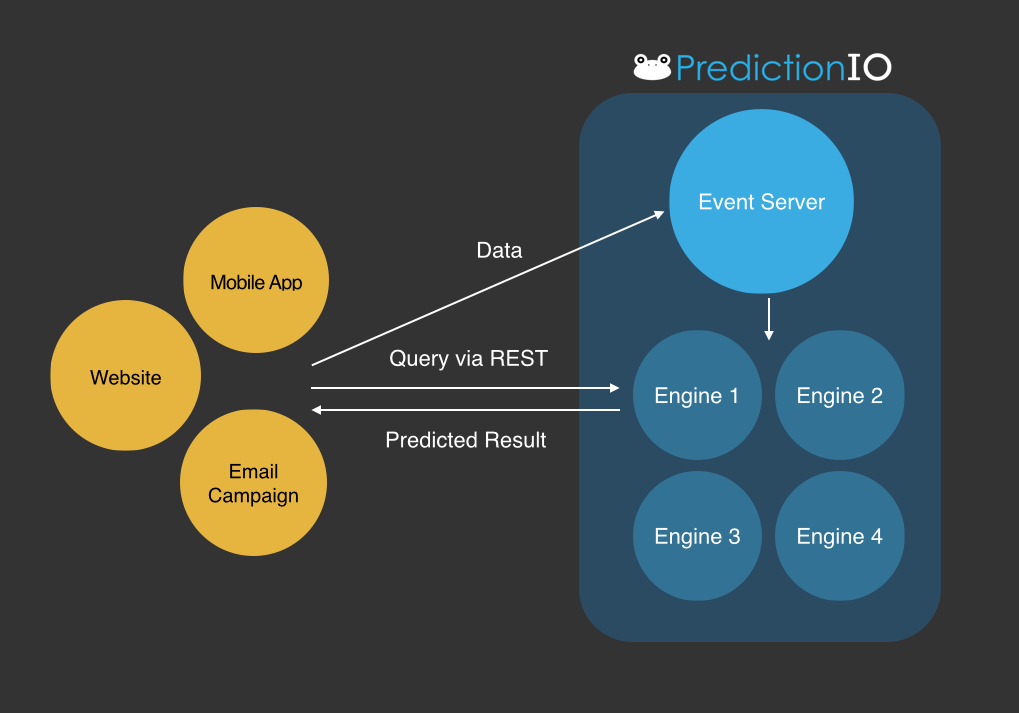
\includegraphics[scale=0.3]{figures/predictionioeventsever.png}
			\centering
			\caption{PreditionIO Engine interaction with Apps and Prediction Engine}
			\label{fig:predictionio}
		\end{figure}
		\item \textbf{Shiny} : This is an R package and allows for easy to build web applications. It is made of two parts UI script and server script. In Figure it can be seen how Shiny can be implemented to exploit the data mining capabilities of R. Shown in Figure \ref{fig:shinyscaling} how multiple users can access shiny R applications \shortcite{Rshiny}.
		\begin{figure}[H]
			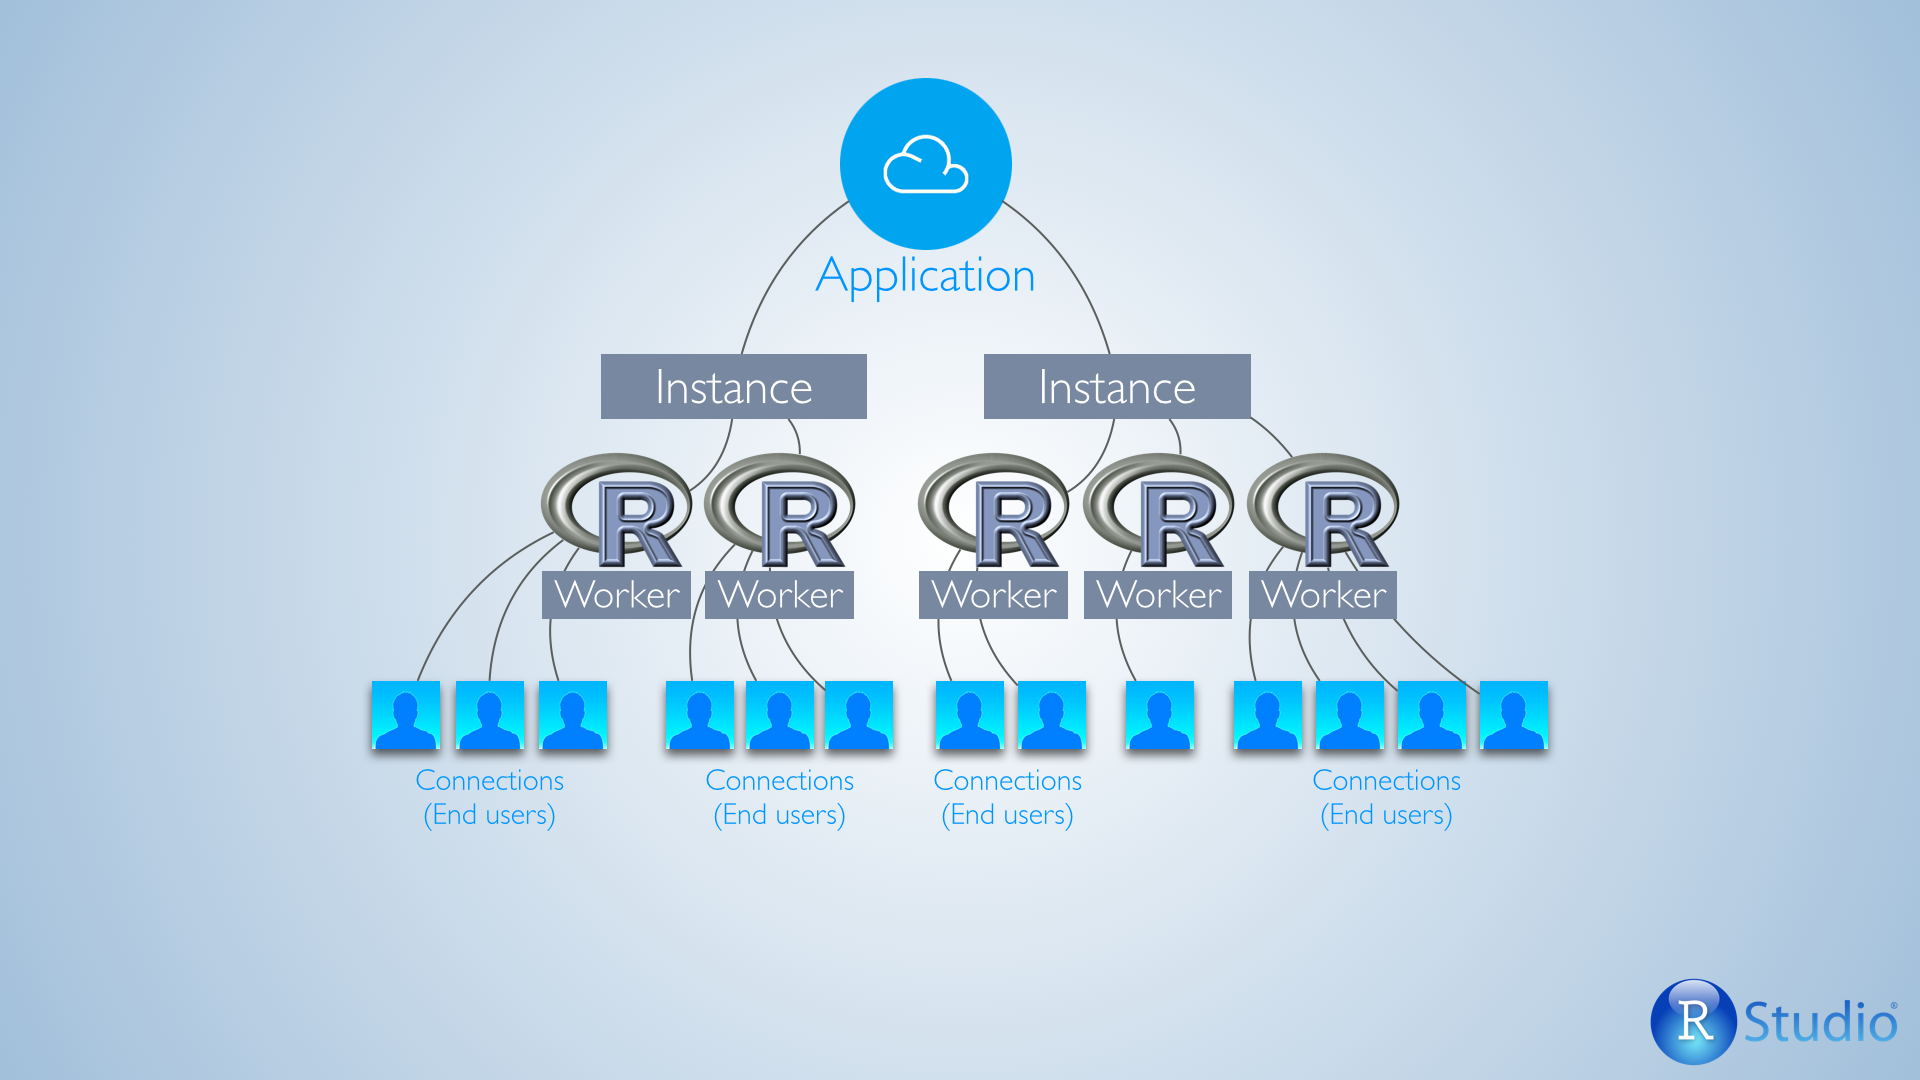
\includegraphics[width=\textwidth,height=10cm]{figures/shinyscaling.png}
			\centering
			\caption{R Shiny architecture}
			\label{fig:shinyscaling}
		\end{figure}
	\end{itemize}
\end{itemize}

\newpage
\section{Model Evaluation Metrics}
Model development is an important process, but evaluations of the model to ascertain its performance is as much an important procedure. The dataset is partitioned suitably and the testing set is not in the view of the model during training. There are however two methods of evaluations.

\begin{itemize}
	\item Holdout technique
	\item K-fold Cross validation technique
	\item Leave one out CV
	\item Bootstrap method
	\item Sensitivity \& Specificity
\end{itemize}

\subsection{Holdout technique}
This method is chosen for evaluation if the dataset is large enough. The data is segregated into three parts viz., Training, Validation and Test sets. 
\begin{itemize}
	\item Training dataset : It is some part of the dataset used for training the models. Predictive models are necessarily trained before actual prediction can be performed eg., Decision Trees, Random forest, Neural network need to be trained.
	\item Validation dataset : This is a subset of the data used to validate the output after model training. It helps to optimize the models performance. It is not mandatory to have validation sets for certain prediction models.
	\item Test dataset : Also a part of the whole dataset, it helps to  
\end{itemize}

\subsection{k-fold cross validation technique}
This method of evaluations is chosen if the dataset is small and limited. The data is partitioned into k equal sized sets with an unbiased process. The model is built k times, with every K-1 data sets selected as training set, leaving out 1 set to be used as test set. A round robin process is followed to select the testing set in every iteration.


\subsection{Sensitivity \& Specificity}
For calculating the performance of the model, a confusion matrix is plotted. The matrix is a cross table between predicted values and the actual values Figure \ref{fig:ConfusionMatrix}.  There are generally four types of values that can be calculated from the matrix and those are as follows :
\begin{itemize}
	\item TP - true positives : The predictor predicts ``True'' for actual true value of data. 
	\item TN - true negatives : The predictor predicts ``False'' for actual false values of data. 
	\item FP - false positives : The predictor predicts ``False'' for actual true value of data.
	\item FN - false negatives : The predictor predicts ``True'' for actual false values of data.
\end{itemize}

\textbf{Sensitivity :} the ratio of the count of the True Positives to the total count of events. This is also called the \textit{\textbf{Recall}}.
\[
	Sensitivity(or Recall) = \frac{TP}{TP+FN}
\]
\\
\textbf{Specificity :} the ratio of the count of the True Negatives to the total count of non-events.
\[
Specificity = \frac{TN}{FP+TN}
\]

In addition to the above, True Positive value is called the \textit{\textbf{Precision}}. 

Form the values of \textit{Precision} and \textit{Recall} another statistical measurement called F-score can be derived.
\[
	F = 2 \times \frac{precision \times recall}{precision + recall}
\]

\begin{figure}[h]
	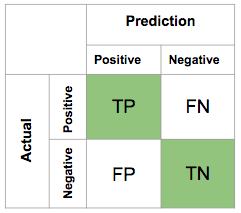
\includegraphics[scale=0.7]{figures/confusionmatrix.png}
	\centering
	\caption{Confusion Matrix}
	\label{fig:ConfusionMatrix}
\end{figure}




\newpage
\section{Review of Selected Research Papers}

In the paper titled `` Modeling \& Simulation  of a Predictive Customer Churn Model for Telecommunication Industry‘’ the authors emulated a neuro fuzzy inference system to study the customer churn in the telecom industry \shortcite{O2015}. They modeled membership functions for the attributes of the dataset. Then they employed search algorithm for feature selection of the variables that indicate churn. Thereafter they model fuzzy equations to relate the dependent variables to the independent variables. This fuzzy system is trained to tune the Adaptive neuro fuzzy system based on the Sugeno FIS. The call detail records of 5000 subscribers was used to model this FIS. The dataset has 21 attributes but here they selected 9. Then the variables were modeled into three categories. For performance evaluation they calculated the Precision rate and the recall rate. After the testing it was found that accuracy was 95.8\% , precision 80.86\%, recall 92.7\%.

A research study ``A Hybrid Churn Prediction Model 
in
Mobile 
Telecommunication Industry '' \shortcite{olle2014hybrid} presents a combination of LR and VP method. The academics used two algorithms of supervised learning viz., Logistic regression and Voted perceptron. They then combined the two into a Hybrid model for classification in WEKA.
The obtained the data from an Asian telcom operator, records of around 2000 customers and 23 attributes.\\
From the results it was observed that hybrid model performed better than each of them individually.

In the study ``A comparison of machine learning techniques for customer churn prediction'' by \shortcite{vafeiadis2015comparison} the researchers present a well meted out comparison between the normal model functions and their corresponding boosted models. The performance criteria was based on the F-score. They had used a series of simulations based on the Monte Carlo method. The models selected for analysis were Back-Propagation algorithm , Support Vector Machines, Decision Trees, Naive Bayes and Logistic Regression. The data was obtained from the publicly available churn dataset hosted at UCI Machine learning repository. The 100-fold cross validation technique was used to reduce bias. Ratio of training to testing set is about $2:3$. A type of the most common boosting algorithm Adaboost, \textit{Adaboost.M1} with DT and BPN as weak classifier was used.\\
The R programming was used for modeling the simulation experiment. Two steps were followed : Step 1 - tested classifiers run with data and performance of F-score measured. Step 2 - boosting algorithm was applied and performance F-score measured. 100 Monte carlo realizations were generated for cross validation of results. Monte carlo is synthesis of datasets that resemble the actual data. It was derieved from the results that two prediction models performed the best. 2 layer BPN with 15 hidden nodes and Decision tree classifier. An accuracy of 94\% and F-measure around 77\%. The SVM scored lower followed by Naive Bayes and Logit Regression at last. After application of the Boosting algo, SVM reported the best accuracy of 97\% and Fmeasure over 84\%.


\begin{landscape}
\section{Summary of Selected Research Studies}
Here some of the past relevant literature in the domain of churn prediction and the results are discussed in Table \ref{table1}.

\begin{longtable}{ | p{20pt} | p{100pt} | p{100pt} | p{150pt} | p{100pt} | p{150pt} | }
	\caption{ Previous literature review}\label{table1}\\
 	
 	\hline
 	SNo & Title \& Author & Objective &  Data \& Methodology & Outcome & Further Research\\
 	\hline
 	\endfirsthead
 	
 	\hline
 	SNo & Title \& Author &Objective & Data \& Methodology &Outcome & Further Research\\
 	\hline
 	\endhead
 	\hline
 	\endfoot
 	\hline
    \endlastfoot
    \hline
    1    % .......................... New Entry
    &
    Modeling \& Simulation  of a Predictive Customer Churn Model for Telecommunication Industry \shortcite{O2015}
    &
    Adaptive neuro fuzzy inference system for prediction emulation of customer churn Neural network + fuzzy logic.
    &
    \textbf{Data :} 5000 subscribers CDR – call detail record with 21 vriables. Partitioned into 5 sets each containing 1000 records.
    \newline
    \textbf{Method :} Number of predictor variables taken is 9. Target variable is Chrun with value Y or N. Membership function for each variable.
    &
    Found that 3 variables are very important. 
    Total no of minute calls, no of customer service calls, no of repaired calls.
    Fuzzy churn model Precison 80.86\% recall 92.7\% and predicted accuracy 95.8\%.
    &
    None suggested
    \\\hline
    2    % .......................... New Entry
    &
    A Hybrid Churn Prediction Model in Mobile Telecommunication Industry \shortcite{olle2014hybrid}
    &
    A model combined with VotedPerceptron and Logisti Regression is performance compared to the models of VP and LR as individual predictors.
    &
    \textbf{Data :} 2000 customers CDR from an Asian telecom company with 23 attributes.
    \textbf{Method :} A hybrid model of VP and LR was used. WEKA tool was used to model.
    &
    The hybrid model performs better than the models prediction accuracy seperately.
    & None suggested
    \\\hline
 	  	 3    % .......................... New Entry
 	  	 &
 	  	 A comparison of machine learning techniques for customer churn prediction \shortcite{vafeiadis2015comparison}
 	  	 &
	  	 The normal model functions were performance compared to their corresponding boosted models.
 	  	 &
 	  	 \textbf{Data :} publicly hosted churn dataset at UCI machine learning repository.
 	  	 \newline
 	  	 \textbf{Method :} Machine learning techniques of Back-Propagation algorithm , Support Vector Machines, Decision Trees, Naive Bayes and Logistic Regression were used. The boosting algorithm Adaboost.M1 a type of Adaboost was used. R progamming was used for modeling the system.
 	  	 &
 	  	 2 prediction models performed the best : 2-layer BPN with 15 hidden nodes and Decision tree classifier. SVM scored lower followed by Naive Bayes and Logit Regression at last. After application of the Boosting algo, SVM reported the best accuracy of 97\% and Fmeasure over 84\%.
 	  	 & None suggested
 	  	 \\\hline
 	 
 	 4    % .......................... New Entry
 	 &
 	 Turning telecommunications call details to churn prediction: a data mining approach \shortcite{wei2002turning}
 	 &
 	 The company experiences a high monthly churn rate of 1.5 – 2%. 
 	 Neural network requires a long time due to it’s iterative nature.
 	 Highly skewed class distribution between churners and non-churners.
 	 &
 	 \textbf{Data :} Telecom company of Taiwan. Contractual and call details of subscribers Oct 2000 – Jan 2001. 9100000 records.
 	 \newline
 	 \textbf{Method : } Multi classifier class combiner, Decision tree C4.5 
 	 &
 	 Churn prediction is relatively high within 1 month duration. Multi classifier performs better than single classifier. 
 	 &
     To include more variables from logs and complaints. Evaluation of empirical stats between customers from different geographic locations. Integration with data-warehouse for constantly learning behavior of customer. Research with other industry data from credit card to Internet service providers.
 	 \\\hline
 	 5    % .......................... New Entry
 	 &
 	 Applying Fuzzy Data Mining to Telecom Churn Management \shortcite{liao2011applying}.
 	 &
 	 To determine the most effective marketing strategies of customer retention, by analyzing the responses of customers. 
 	 &
 	 \textbf{Data :} Taiwan telecom company, retention activity \& response data for customer contract expiry between June and Junly 2008
 	 \newline
 	 \textbf{Method : } ID3 decision tree for classification.
 	 &
 	 Using fuzzy set the customer retention shows that marketing via telemarketing is more  effective compared with Direct mailing.
 	 Also fuzzy marketing technique is better than direct mailing marketing for customers with higher bill amounts.
 	 &
 	 Fuzzy data mining techniques to analyze the past records of results of various marketing activities to establish a marketing mode.
 	 \\\hline
 	 6    % .......................... New Entry
 	 & 
 	 Customer churn prediction using improved balanced random forests \shortcite{xie2009customer}.
 	 &
 	 a novel learning method, called improved balanced random forests (IBRF), and demonstrate its application to churn prediction
 	 &
 	 \textbf{Data :} Chinese bank data. 1524 [762 train, 762 test].
 	 \newline
 	 \textbf{Method : } IBRF = Balanced random forest + weighted random forest. 
 	 Introduce 2 interval variables ‘m – middle pt’ \& ‘d – length of interval’. 
 	 apply IBRF to a set of churn data in a bank as test the performance of our proposed method, we run several comparative experiments comparison of results from IBRF and other standard methods, namely artificial neural network (ANN), decision tree (DT), and CWC-SVM (Scholkopf, Platt, Shawe, Smola, \& Williamson,
 	 &
 	 Accuracy rate follows this pattern \(IBRF > CWC-SVM > ANN > DT\),
 	 Top-decile Lift varies as this \(IBRF > CWV-SVM > DT > ANN\).
 	 IBRF offers great potential compared to traditional approaches due to its scalability, and faster training and running speeds.
 	 &
 	 Experimenting with some other weak learners in random forests. Improving effectiveness and generalization ability.
 	 \\\hline
 	 7    % .......................... New Entry
 	 &
 	 Churn prediction in subscription services: An application of support vector machines while comparing two parameter-selection techniques \shortcite{coussement2008churn}
 	 &
 	 Churn prediction using SVM. Benchmarked to Logit regression and random forest.
 	 &
 	 \textbf{Data :} Belgian newspaper publishing  company. Training set 45000, Test set 45000
 	 \newline
 	 \textbf{Method : } Use of random forest software and SVM-toolbox. SVM compared to Logit regression \& random forest. 
 	 Grid search using 5-fold cross-validation
 	 &
 	 SVM trained on balanced distribution, outperforms logit regression when parameter selection applied. Random forest surpass SVM. Academincs and practionerx don’t need to rely on traditional Logit reg, SVM with parameter selection technique and random forest offer better alternative
 	 &
 	 No complete working meta-theory to choose kernel function and SVM parameters. Thus deriving a procedure to select proper kernel function and SVM parameter.
 	 \\\hline
 	 8    % .......................... New Entry
 	 &
 	 Customer churn prediction by Hybrid neural networks \shortcite{tsai2009customer}
 	 &
 	 Very few studies for hybrid data mining appraoch for prediction.
 	 &
 	 \textbf{Data :} CRM dataset from American telephone company, July 2001 to Jan 2002 51,306 subscribers.
 	 \newline
 	 \textbf{Method : } 2 methods developed and compared for performance. M1 – SOM + ANN clustering + classification is used. M2 – ANN + ANN 2 classifiers are used. 5 fold cross validation, each set of the 5 are tested 5 times. Baseline is 20 ANN’s
 	 &
 	 Baseline ANN models had prediction accuracy of 88\%
 	 performance : $ANN + ANN > single ANN$\newline
 	 $3*3$ SOM is best among $2*2$ , $3*3$, $4*4$ and $5*5$ clustering 
 	 Performance of the hybrid models is : $ANN + ANN > SOM + ANN > ANN$
 	 &
 	 Need to explore dimensionality reduction or Feature selection of data preprocessing. Application of SVM or genetic algorithms. Explore other domains for churn prediction.
 	 \\\hline
 	 9    % .......................... New Entry
 	 &
 	 Predicting customer retention and profitability by using random forest and regression forest \shortcite{lariviere2005predicting}
 	 &
 	 The paper discusses more than one variable of retention and profit outcome.
 	 &
 	 \textbf{Data :} 100,000 Belgian finance company. Divided into 2 random parts, one for estimation other for evaluation.
 	 \newline
 	 \textbf{Method :} Authors used random forest for regression to predict profitability,  next purchase and defection decision. Benchmarked to linear regression model.
 	 &
 	 Random forest are better than logit and linear regression.
 	 &
 	 None suggested.
 	 \\\hline
 	 10    % .......................... New Entry
 	 &
 	 Churn prediction using comprehensible support vector machine: An analytical CRM application
 	 &
 	 The paper discusses more than one variable of retention and profit outcome.
 	 &
 	 \textbf{Data :} 100,000 Belgian finance company. Divided into 2 random parts, one for estimation other for evaluation.
 	 \newline
 	 \textbf{Method :} Authors used random forest for regression to predict profitability,  next purchase and defection decision. Benchmarked to linear regression model.
 	 &
 	 Random forest are better than logit and linear regression.
 	 &
 	 None suggested.
 	 \\\hline
 	 11    % .......................... New Entry
 	 &
 	 Churn prediction for high-value players in casual social games
 	 &
 	 Paper presents churn prediction of players of social games and the business impact of retaining high valued players.
 	 &
 	 \textbf{Data :} dataset of high value users of games - Diamond dash and Monster World, for 2 days. 
 	 \newline
 	 \textbf{Method :} The researchers trained and predicted neural networks, logistic regression, decision tree and support vector machine. Radial basis function for support vector machine was used with 10-fold cross validation. For business impact of churning the researchers designed A/B test.	 
 	 &
 	 Single neural network with tuned learning rate is better that other algorithms. A/B test reveals that sending free coins to high value customers does not affect churn rate.
 	 &
 	 None suggested.
 	 
 \end{longtable}

\end{landscape}

\FloatBarrier

